

\tikzset{every picture/.style={line width=0.75pt}} %set default line width to 0.75pt        

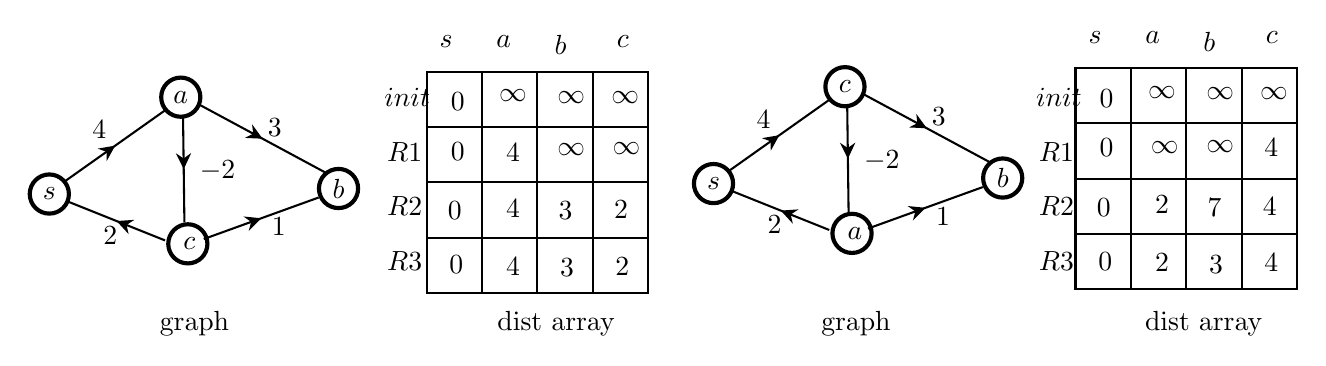
\begin{tikzpicture}[x=0.5pt,y=0.5pt,yscale=-1,xscale=1]
%uncomment if require: \path (0,238); %set diagram left start at 0, and has height of 238

%Straight Lines [id:da6460204159880261] 
\draw [color={rgb, 255:red, 0; green, 0; blue, 0 }  ,draw opacity=1 ][line width=0.75]    (44,115) -- (116,64) ;
\draw [shift={(80,89.5)}, rotate = 144.69] [fill={rgb, 255:red, 0; green, 0; blue, 0 }  ,fill opacity=1 ][line width=0.08]  [draw opacity=0] (11.61,-5.58) -- (0,0) -- (11.61,5.58) -- (7.71,0) -- cycle    ;
%Straight Lines [id:da6066395504516056] 
\draw [color={rgb, 255:red, 0; green, 0; blue, 0 }  ,draw opacity=1 ][line width=0.75]    (46,130) -- (116,158) ;
\draw [shift={(81,144)}, rotate = 21.8] [fill={rgb, 255:red, 0; green, 0; blue, 0 }  ,fill opacity=1 ][line width=0.08]  [draw opacity=0] (11.61,-5.58) -- (0,0) -- (11.61,5.58) -- (7.71,0) -- cycle    ;
%Straight Lines [id:da1865492813606927] 
\draw [color={rgb, 255:red, 0; green, 0; blue, 0 }  ,draw opacity=1 ][line width=0.75]    (227,127) -- (144,157) ;
\draw [shift={(185.5,142)}, rotate = 160.13] [fill={rgb, 255:red, 0; green, 0; blue, 0 }  ,fill opacity=1 ][line width=0.08]  [draw opacity=0] (11.61,-5.58) -- (0,0) -- (11.61,5.58) -- (7.71,0) -- cycle    ;
%Straight Lines [id:da7037921758898328] 
\draw [color={rgb, 255:red, 0; green, 0; blue, 0 }  ,draw opacity=1 ][line width=0.75]    (232,109) -- (141,60) ;
\draw [shift={(186.5,84.5)}, rotate = 208.3] [fill={rgb, 255:red, 0; green, 0; blue, 0 }  ,fill opacity=1 ][line width=0.08]  [draw opacity=0] (11.61,-5.58) -- (0,0) -- (11.61,5.58) -- (7.71,0) -- cycle    ;
%Straight Lines [id:da8291596598765129] 
\draw [color={rgb, 255:red, 0; green, 0; blue, 0 }  ,draw opacity=1 ][line width=0.75]    (129,68) -- (130,145) ;
\draw [shift={(129.5,106.5)}, rotate = 269.26] [fill={rgb, 255:red, 0; green, 0; blue, 0 }  ,fill opacity=1 ][line width=0.08]  [draw opacity=0] (11.61,-5.58) -- (0,0) -- (11.61,5.58) -- (7.71,0) -- cycle    ;
%Shape: Grid [id:dp9545383501398971] 
\draw  [draw opacity=0] (305,36) -- (465,36) -- (465,196) -- (305,196) -- cycle ; \draw   (345,36) -- (345,196)(385,36) -- (385,196)(425,36) -- (425,196) ; \draw   (305,76) -- (465,76)(305,116) -- (465,116)(305,156) -- (465,156) ; \draw   (305,36) -- (465,36) -- (465,196) -- (305,196) -- cycle ;
%Straight Lines [id:da6859977927436415] 
\draw [color={rgb, 255:red, 0; green, 0; blue, 0 }  ,draw opacity=1 ][line width=0.75]    (524,107.44) -- (596,56.44) ;
\draw [shift={(560,81.94)}, rotate = 144.69] [fill={rgb, 255:red, 0; green, 0; blue, 0 }  ,fill opacity=1 ][line width=0.08]  [draw opacity=0] (11.61,-5.58) -- (0,0) -- (11.61,5.58) -- (7.71,0) -- cycle    ;
%Straight Lines [id:da7933127864023365] 
\draw [color={rgb, 255:red, 0; green, 0; blue, 0 }  ,draw opacity=1 ][line width=0.75]    (526,122.44) -- (596,150.44) ;
\draw [shift={(561,136.44)}, rotate = 21.8] [fill={rgb, 255:red, 0; green, 0; blue, 0 }  ,fill opacity=1 ][line width=0.08]  [draw opacity=0] (11.61,-5.58) -- (0,0) -- (11.61,5.58) -- (7.71,0) -- cycle    ;
%Straight Lines [id:da4572703425075384] 
\draw [color={rgb, 255:red, 0; green, 0; blue, 0 }  ,draw opacity=1 ][line width=0.75]    (707,119.44) -- (624,149.44) ;
\draw [shift={(665.5,134.44)}, rotate = 160.13] [fill={rgb, 255:red, 0; green, 0; blue, 0 }  ,fill opacity=1 ][line width=0.08]  [draw opacity=0] (11.61,-5.58) -- (0,0) -- (11.61,5.58) -- (7.71,0) -- cycle    ;
%Straight Lines [id:da6555386770352928] 
\draw [color={rgb, 255:red, 0; green, 0; blue, 0 }  ,draw opacity=1 ][line width=0.75]    (712,101.44) -- (621,52.44) ;
\draw [shift={(666.5,76.94)}, rotate = 208.3] [fill={rgb, 255:red, 0; green, 0; blue, 0 }  ,fill opacity=1 ][line width=0.08]  [draw opacity=0] (11.61,-5.58) -- (0,0) -- (11.61,5.58) -- (7.71,0) -- cycle    ;
%Straight Lines [id:da10548541378466969] 
\draw [color={rgb, 255:red, 0; green, 0; blue, 0 }  ,draw opacity=1 ][line width=0.75]    (609,60.44) -- (610,137.44) ;
\draw [shift={(609.5,98.94)}, rotate = 269.26] [fill={rgb, 255:red, 0; green, 0; blue, 0 }  ,fill opacity=1 ][line width=0.08]  [draw opacity=0] (11.61,-5.58) -- (0,0) -- (11.61,5.58) -- (7.71,0) -- cycle    ;
%Shape: Grid [id:dp20210036402389486] 
\draw  [draw opacity=0] (774,33.44) -- (934,33.44) -- (934,193.44) -- (774,193.44) -- cycle ; \draw   (814,33.44) -- (814,193.44)(854,33.44) -- (854,193.44)(894,33.44) -- (894,193.44) ; \draw   (774,73.44) -- (934,73.44)(774,113.44) -- (934,113.44)(774,153.44) -- (934,153.44) ; \draw   (774,33.44) -- (934,33.44) -- (934,193.44) -- (774,193.44) -- cycle ;

% Text Node
\draw (69.24,145.53) node [anchor=north west][inner sep=0.75pt]   [align=left] {$\displaystyle 2$};
% Text Node
\draw  [line width=1.5]   (32.38, 124.47) circle [x radius= 14.15, y radius= 14.15]   ;
\draw (32.38,124.47) node   [align=left] {$\displaystyle s$};
% Text Node
\draw  [line width=1.5]   (127.38, 54.47) circle [x radius= 14.15, y radius= 14.15]   ;
\draw (127.38,54.47) node   [align=left] {$\displaystyle a$};
% Text Node
\draw  [line width=1.5]   (132.48, 160.47) circle [x radius= 14.15, y radius= 14.15]   ;
\draw (126.98,160.47) node [anchor=west] [inner sep=0.75pt]   [align=left] {$\displaystyle c$};
% Text Node
\draw  [line width=1.5]   (241.38, 120.47) circle [x radius= 14.15, y radius= 14.15]   ;
\draw (241.38,120.47) node   [align=left] {$\displaystyle b$};
% Text Node
\draw (61.24,69.53) node [anchor=north west][inner sep=0.75pt]   [align=left] {$\displaystyle 4$};
% Text Node
\draw (188,67.47) node [anchor=north west][inner sep=0.75pt]   [align=left] {$\displaystyle 3$};
% Text Node
\draw (191,139.47) node [anchor=north west][inner sep=0.75pt]   [align=left] {$\displaystyle 1$};
% Text Node
\draw (139,98.47) node [anchor=north west][inner sep=0.75pt]   [align=left] {$\displaystyle -2$};
% Text Node
\draw (320.24,49.06) node [anchor=north west][inner sep=0.75pt]   [align=left] {$\displaystyle 0$};
% Text Node
\draw (274.24,85.23) node [anchor=north west][inner sep=0.75pt]   [align=left] {$\displaystyle R1$};
% Text Node
\draw (312.24,7.56) node [anchor=north west][inner sep=0.75pt]   [align=left] {$\displaystyle s$};
% Text Node
\draw (353.24,7.56) node [anchor=north west][inner sep=0.75pt]   [align=left] {$\displaystyle a$};
% Text Node
\draw (395.24,7.56) node [anchor=north west][inner sep=0.75pt]   [align=left] {$\displaystyle b$};
% Text Node
\draw (440.24,7.56) node [anchor=north west][inner sep=0.75pt]   [align=left] {$\displaystyle c$};
% Text Node
\draw (355.24,47.06) node [anchor=north west][inner sep=0.75pt]   [align=left] {$\displaystyle \infty $};
% Text Node
\draw (397.24,48.06) node [anchor=north west][inner sep=0.75pt]   [align=left] {$\displaystyle \infty $};
% Text Node
\draw (436.24,48.06) node [anchor=north west][inner sep=0.75pt]   [align=left] {$\displaystyle \infty $};
% Text Node
\draw (272.24,46.06) node [anchor=north west][inner sep=0.75pt]   [align=left] {$\displaystyle init$};
% Text Node
\draw (320.24,85.06) node [anchor=north west][inner sep=0.75pt]   [align=left] {$\displaystyle 0$};
% Text Node
\draw (360.24,86.06) node [anchor=north west][inner sep=0.75pt]   [align=left] {$\displaystyle 4$};
% Text Node
\draw (360.24,126.06) node [anchor=north west][inner sep=0.75pt]   [align=left] {$\displaystyle 4$};
% Text Node
\draw (360.24,168.06) node [anchor=north west][inner sep=0.75pt]   [align=left] {$\displaystyle 4$};
% Text Node
\draw (318.24,128.06) node [anchor=north west][inner sep=0.75pt]   [align=left] {$\displaystyle 0$};
% Text Node
\draw (319.24,167.06) node [anchor=north west][inner sep=0.75pt]   [align=left] {$\displaystyle 0$};
% Text Node
\draw (398.24,128.06) node [anchor=north west][inner sep=0.75pt]   [align=left] {$\displaystyle 3$};
% Text Node
\draw (399.24,169.06) node [anchor=north west][inner sep=0.75pt]   [align=left] {$\displaystyle 3$};
% Text Node
\draw (439.24,168.06) node [anchor=north west][inner sep=0.75pt]   [align=left] {$\displaystyle 2$};
% Text Node
\draw (438.24,127.06) node [anchor=north west][inner sep=0.75pt]   [align=left] {$\displaystyle 2$};
% Text Node
\draw (274.24,124.4) node [anchor=north west][inner sep=0.75pt]   [align=left] {$\displaystyle R2$};
% Text Node
\draw (274.24,163.56) node [anchor=north west][inner sep=0.75pt]   [align=left] {$\displaystyle R3$};
% Text Node
\draw (110,206.72) node [anchor=north west][inner sep=0.75pt]   [align=left] {graph};
% Text Node
\draw (354,206.72) node [anchor=north west][inner sep=0.75pt]   [align=left] {dist array};
% Text Node
\draw (397.24,86.06) node [anchor=north west][inner sep=0.75pt]   [align=left] {$\displaystyle \infty $};
% Text Node
\draw (437.24,85.06) node [anchor=north west][inner sep=0.75pt]   [align=left] {$\displaystyle \infty $};
% Text Node
\draw (549.24,137.97) node [anchor=north west][inner sep=0.75pt]   [align=left] {$\displaystyle 2$};
% Text Node
\draw  [line width=1.5]   (512.38, 116.91) circle [x radius= 14.15, y radius= 14.15]   ;
\draw (512.38,116.91) node   [align=left] {$\displaystyle s$};
% Text Node
\draw  [line width=1.5]   (607.38, 46.91) circle [x radius= 14.15, y radius= 14.15]   ;
\draw (607.38,46.91) node   [align=left] {$\displaystyle c$};
% Text Node
\draw  [line width=1.5]   (612.48, 152.91) circle [x radius= 14.15, y radius= 14.15]   ;
\draw (606.98,152.91) node [anchor=west] [inner sep=0.75pt]   [align=left] {$\displaystyle a$};
% Text Node
\draw  [line width=1.5]   (721.38, 112.91) circle [x radius= 14.15, y radius= 14.15]   ;
\draw (721.38,112.91) node   [align=left] {$\displaystyle b$};
% Text Node
\draw (541.24,61.97) node [anchor=north west][inner sep=0.75pt]   [align=left] {$\displaystyle 4$};
% Text Node
\draw (668,59.91) node [anchor=north west][inner sep=0.75pt]   [align=left] {$\displaystyle 3$};
% Text Node
\draw (671,131.91) node [anchor=north west][inner sep=0.75pt]   [align=left] {$\displaystyle 1$};
% Text Node
\draw (619,90.91) node [anchor=north west][inner sep=0.75pt]   [align=left] {$\displaystyle -2$};
% Text Node
\draw (789.24,46.5) node [anchor=north west][inner sep=0.75pt]   [align=left] {$\displaystyle 0$};
% Text Node
\draw (781.24,5) node [anchor=north west][inner sep=0.75pt]   [align=left] {$\displaystyle s$};
% Text Node
\draw (822.24,5) node [anchor=north west][inner sep=0.75pt]   [align=left] {$\displaystyle a$};
% Text Node
\draw (864.24,5) node [anchor=north west][inner sep=0.75pt]   [align=left] {$\displaystyle b$};
% Text Node
\draw (909.24,5) node [anchor=north west][inner sep=0.75pt]   [align=left] {$\displaystyle c$};
% Text Node
\draw (824.24,44.5) node [anchor=north west][inner sep=0.75pt]   [align=left] {$\displaystyle \infty $};
% Text Node
\draw (866.24,45.5) node [anchor=north west][inner sep=0.75pt]   [align=left] {$\displaystyle \infty $};
% Text Node
\draw (905.24,45.5) node [anchor=north west][inner sep=0.75pt]   [align=left] {$\displaystyle \infty $};
% Text Node
\draw (789.24,82.5) node [anchor=north west][inner sep=0.75pt]   [align=left] {$\displaystyle 0$};
% Text Node
\draw (908.24,82.5) node [anchor=north west][inner sep=0.75pt]   [align=left] {$\displaystyle 4$};
% Text Node
\draw (829.24,123.5) node [anchor=north west][inner sep=0.75pt]   [align=left] {$\displaystyle 2$};
% Text Node
\draw (829.24,165.5) node [anchor=north west][inner sep=0.75pt]   [align=left] {$\displaystyle 2$};
% Text Node
\draw (787.24,125.5) node [anchor=north west][inner sep=0.75pt]   [align=left] {$\displaystyle 0$};
% Text Node
\draw (788.24,164.5) node [anchor=north west][inner sep=0.75pt]   [align=left] {$\displaystyle 0$};
% Text Node
\draw (867.24,125.5) node [anchor=north west][inner sep=0.75pt]   [align=left] {$\displaystyle 7$};
% Text Node
\draw (868.24,166.5) node [anchor=north west][inner sep=0.75pt]   [align=left] {$\displaystyle 3$};
% Text Node
\draw (908.24,165.5) node [anchor=north west][inner sep=0.75pt]   [align=left] {$\displaystyle 4$};
% Text Node
\draw (907.24,124.5) node [anchor=north west][inner sep=0.75pt]   [align=left] {$\displaystyle 4$};
% Text Node
\draw (588,206.72) node [anchor=north west][inner sep=0.75pt]   [align=left] {graph};
% Text Node
\draw (822,206.72) node [anchor=north west][inner sep=0.75pt]   [align=left] {dist array};
% Text Node
\draw (866.24,83.5) node [anchor=north west][inner sep=0.75pt]   [align=left] {$\displaystyle \infty $};
% Text Node
\draw (826.24,84.5) node [anchor=north west][inner sep=0.75pt]   [align=left] {$\displaystyle \infty $};
% Text Node
\draw (745.24,85.23) node [anchor=north west][inner sep=0.75pt]   [align=left] {$\displaystyle R1$};
% Text Node
\draw (743.24,46.06) node [anchor=north west][inner sep=0.75pt]   [align=left] {$\displaystyle init$};
% Text Node
\draw (745.24,124.4) node [anchor=north west][inner sep=0.75pt]   [align=left] {$\displaystyle R2$};
% Text Node
\draw (745.24,163.56) node [anchor=north west][inner sep=0.75pt]   [align=left] {$\displaystyle R3$};


\end{tikzpicture}

